%%%%%%%%%%%%%%%%%%%%%%%%%%%%%%%%%%%%%%%%%%%%%%%%%%%%%%%%%%%%%%%%%%%%%%%%%
%%   CHAPTER: UNIVERSAL CONSTRUCTION
%%%%%%%%%%%%%%%%%%%%%%%%%%%%%%%%%%%%%%%%%%%%%%%%%%%%%%%%%%%%%%%%%%%%%%%%%

\renewcommand{\chapterfolder}{universal_construction/}
\chapterimage{cover/universal_construction}
\chapter{Universal Construction}\label{chp:universal_construction}


\vspace*{-0.4in}
\epigraph{The truth is you don't know what is going to happen tomorrow. Life is a crazy ride, and nothing is guaranteed.}{Eminem}
\vspace*{0.4in}


\noindent In the previous chapter, we learned that we can often stabilize unstable reactions (like the $31c/240$~reaction of Figure~\ref{fig:31c_240_reaction}, or the $17c/45$~reaction of Figure~\ref{fig:17c45_reaction}) by using them to create gliders, and then using those gliders to synthesize stabilizing components. In this chapter, we take this idea one step further and show that similar behavior can be achieved without the need for the initial unstable reaction---we can use gliders to create or move some component in the Life plane, while simultaneously moving or recreating those gliders so that they can be re-used.

% Some paragraph about what makes construction 'Universal" -- anything that can be glider constructed can be constructed via these mechanisms. Maybe footnote that it is not known if every non-GoE is glider constructible.


%%%%%%%%%%%%%%%%%%%%%%%%%%%%%%%%
\section{Gemini}\label{sec:gemini}\index{gemini}
%%%%%%%%%%%%%%%%%%%%%%%%%%%%%%%%

We have seen the basic idea behind universal construction several times now, starting back in Section~\ref{sec:slide_guns}. By using a sliding block (or other small still life) as an elbow, we can fire gliders at any location in the Life plane, thus allowing a sequence of gliders to encode the construction or destruction of essentially any pattern (via the slow salvo techniques of Section~\ref{sec:slow_salvo}, for example).

We already saw gliders salvos that push or pull a sliding block back in Figure~\ref{fig:synchronized_block_movers}, as well as salvos that can be used to fire perpendicular gliders of either color in Figure~\ref{fig:synchronized_block_reflectors}. We summarize those reactions that we will make use of in Figure~\ref{fig:gemini_glider_operations},\footnote{The names ``\texttt{FIRE WHITE}'' and ``\texttt{FIRE BLACK}'' used for two of these reactions just refer to the fact that they fire perpendicular gliders of opposite colors (the absolute color names do not matter).} noting that just these four operations are enough for us to be able to implement any unidirectional slow salvo of our choosing.% Footnote about only needing 3?

\begin{figure}[!htb]
	\centering
	\begin{tabular}{@{}cccc@{}}
		\begin{subfigure}{0.23\textwidth}
			\centering
			\patternimglink{0.12}{gemini_pull}
			\caption{\texttt{PULL}}
			\label{fig:gemini_pull}
		\end{subfigure} & \begin{subfigure}{0.23\textwidth}
			\centering
			\patternimglink{0.12}{gemini_push}
			\caption{\texttt{PUSH}}
			\label{fig:gemini_push}
		\end{subfigure} & \begin{subfigure}{0.23\textwidth}
			\centering
			\patternimglink{0.12}{gemini_fire_white}
			\caption{\texttt{FIRE WHITE}}
			\label{fig:gemini_fire_white}
		\end{subfigure} & \begin{subfigure}{0.23\textwidth}
			\centering
			\patternimglink{0.12}{gemini_fire_black}
			\caption{\texttt{FIRE BLACK}}
			\label{fig:gemini_fire_black}
		\end{subfigure}
	\end{tabular}
	\caption{A collection of reactions that can be used to fire perpendicular gliders (to the southwest) along any lane of our choosing. All four reactions use the same initial pair of gliders (highlighted in \bgbox{orangeback2}{orange}).}\label{fig:gemini_glider_operations}
\end{figure}

By using some Herschel circuitry to create these glider configurations, we can straightforwardly construct the component displayed in Figure~\ref{fig:construction_arm} that takes an input glider on one of four different lanes and performs the corresponding operation on  the sliding block. This particular component uses some slightly old conduits like Silver reflectors (refer back to Figure~\ref{fig:silver_reflector}) rather than more recent conduits for two reasons: (1) it will be useful for us to have this component built entirely out of pieces like blocks and eater~1s (and unlike Snarks) that are ``simple'' to synthesize, and (2) the Gemini spaceship that we will construct out of this component was built before many of the more efficient conduits that we have explored.\footnote{For example, the Gemini spaceship that we will soon construct was built in 2010, whereas the Snark was found in 2013 and the syringe was found in 2015.}

\begin{figure}[!htb]
	\centering
	\embedlink{construction_arm}{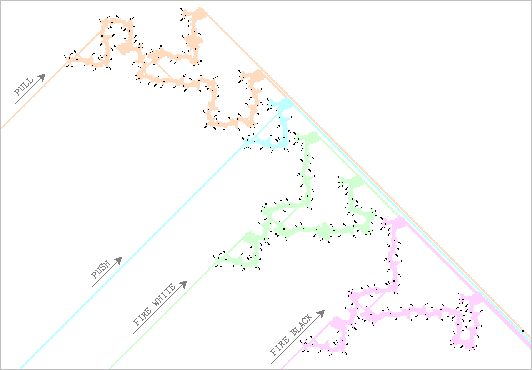
\includegraphics[width=\textwidth]{universal_construction/construction_arm.pdf}}
	\caption{An elbow-operation circuit, which takes a glider on one of four input glider lanes and as a result either pulls or pushes the sliding block (elbow), or uses it to fire a perpendicular glider of either color to the southwest. Note that all four actions require the \texttt{PULL} circuit to be activated, as it produces the frontmost pair of gliders in all four operations (see Exercise~\ref{exer:construction_arm_lanes_timed}). Constructed by Paul Chapman in 2004.}\label{fig:construction_arm}
\end{figure}

By aiming the output gliders of two of these elbow-operation circuits at each other, we can encode the construction of any glider-synthesizable pattern in the input streams (with the advantage that the input lanes are fixed, whereas the output lanes are not).\footnote{This is similar to how we encoded the synthesis of a $2$-engine Cordership in some glider sequences back in Figure~\ref{fig:armless_cordership_gun}.} For example, the pattern displayed in Figure~??...

% FIGURE

Importantly, because these circuits are made up of such simple components (mostly blocks and eater~1s, with the most difficult piece to synthesize being a tub), they can even be used to synthesize copies of \emph{themselves}. Indeed, this is the key idea behind the Gemini: use an extremely long chain of gliders to have two of these circuits build 


%%%%%%%%%%%%%%%%%%%%%%%%%%%%%%%%
\section{Demonoids}\label{sec:demonoid}
%%%%%%%%%%%%%%%%%%%%%%%%%%%%%%%%

Stuff.

\begin{figure}[!htb]
	\centering
	\patternimglink{0.1}{demonoid}
	\caption{A demonoid. Just testing some stuff for now.}\label{fig:demonoid}
\end{figure}



%%%%%%%%%%%%%%%%%%%%%%%%%%%%%%%%
\section*{Notes and Historical Remarks}
%%%%%%%%%%%%%%%%%%%%%%%%%%%%%%%%

Stuff.


% BUILD A GEMINI WITH DIFFERENT PERIOD/SLOPE/WHATEVER
%%%%%%%%%%%%%%%%%%%%%%%%%%%%%%%%%
\section*{Exercises \hfill \normalfont\textsf{\small solutions on \hyperlink{solutions_universal_construction}{page \pageref{solutions_universal_construction}}}}
\label{sec:universal_construction_exercises}
\addcontentsline{toc}{section}{Exercises}
\vspace*{-0.4cm}\hrulefill\vspace*{-0.3cm}\footnotesize\begin{multicols}{2}\vspace*{-0.4cm}\raggedcolumns\interlinepenalty=10000
\setlength{\parskip}{0pt}
%%%%%%%%%%%%%%%%%%%%%%%%%%%%%%%%%


\begin{problem}\label{exer:construction_arm_lanes_timed}
	The elbow-operation circuit of Figure~\ref{fig:construction_arm} requires two synchronized input gliders to trigger each of the \texttt{PUSH}, \texttt{FIRE WHITE}, and \texttt{FIRE BLACK} operations---one to create the frontmost pair of gliders via the \texttt{PULL} circuit, and one to create the additional glider(s).
	
	Add additional Herschel conduits to that circuit so that each of the four operations can be triggered by just a single input glider.
\end{problem}


\mfilbreak


\begin{problem}\label{exer:universal_construction_ex2}
	Another exercise could be placed here.
\end{problem}


%% EXERCISE END COMMANDS
\end{multicols}
\normalsize\vspace*{0.01cm}
%% DONE EXERCISE END COMMANDS